% !TeX program = lualatex
% !TeX encoding = utf8
% !TeX spellcheck = uk_UA
% !BIB program = biber
% !TeX root =../QChemBook.tex
\graphicspath{ {\currfiledir/Pictures/} }

\chapter{Адіабатичне наближення. Ядерна та електронна підсистеми}

Лише невелика кількість задач квантової механіки можуть бути розв'язані математично точно. До таких задач відноситься, наприклад, задача про атом водню. Для систем, які складаються з багатьох частинок (атомів та молекул) точний розрахунок хвильової функції вже неможливий. Якщо відволіктись від проблем, які пов'язані з релятивістськими ефектами, то основна причина, яка не дає точно розв'язати рівняння Шредінґера полягає у взаємодії між електронами, саме наявність оператора міжелектронної взаємодії не дає можливості розділити змінні і отримати точний розв'язок.

Внаслідок цього практична придатність квантової механіки в значній мірі залежить від того, наскільки добре вдасться розробити наближені методи розрахунку хвильової функцій і фізичних величин. Однак, розробка наближених методів ні в якому разі не  обмежується лише завданням чисельно визначити фізичні або фізико-хімічні величини. Ці методи, крім цього, ще й повинні сприяти систематизації та інтерпретації емпіричних даних, розуміння основних закономірностей, формування нових модельних уявлень і розробці на їх основі загальних прогнозів.

Це стосується і прикладанню квантової механіки до проблем хімічного зв'язку і реакційної здатності --- тобто, до квантової хімії. Від результатів квантової хімії слід вимагати, щоб вони відповідали якісним правилам і уявленням про структуру і властивості молекул, які отримані з великого числа експериментальних даних. 

При вивченні станів квантово-механічних систем, зокрема і атомно-мо\-ле\-ку\-лярних, розглядають стаціонарне рівняння Шредінґера:
\begin{equation}\label{eq:Shroedinger_equation}
		\hat{H} \Psi= E \Psi,
\end{equation}
з хвильовими функціями вигляду
\begin{equation}\label{eq:Psi}
    \Psi = \Psi(\vect{r}_1, \sigma_1, \vect{r}_2, \sigma_2, \ldots, \vect{r}_N, \sigma_N; \vect{R}_1, \vect{R_2}, \ldots, \vect{R}_K), 
\end{equation}
де $\vect{r}_i$ та $\sigma_i$~--- просторові та спінові координати електронів, відповідно, $\vect{R}_\alpha$~--- координати ядер, $N$~--- число електронів, $K$~--- число ядер.

Хвильова функція~\eqref{eq:Psi} повинна залежати також і від спінових змінних самих ядер, однак, як правило, в квантовій хімії нехтують цією залежністю.


Гамільтоніан атомно-молекулярної має вигляд:

\begin{multline}\label{eq:H}
    \hat{H} = \hat{T}_{n} + \hat{T}_{e} +  \hat{V}_{nn} + \hat{V}_{en} + \hat{V}_{ee} = \\
    = -\sum\limits_{\alpha = 1}^K \frac{\hbar}{2M_\alpha} \nabla^2_\alpha 
   -\frac{\hbar}{2m} \sum\limits_{i = 1}^N  \nabla^2_i
    + \frac12 \sum\limits_{\alpha \neq \beta}^K \frac{Z_\alpha Z_\beta e^2}{|\vect{R}_\alpha - \vect{R}_\beta|}
    - \sum\limits_{\alpha = 1}^K  \sum\limits_{i = 1}^N \frac{Z_\alpha e^2}{|\vect{R}_\alpha - \vect{r}_i|}
    + \frac12 \sum\limits_{i \neq j}^N \frac{e^2}{|\vect{r}_i - \vect{r}_j|},
\end{multline}
де
$\hat{T}_{n} = -\sum\limits_{\alpha = 1}^K \frac{\hbar}{2M_\alpha} \nabla^2_\alpha $~--- оператор кінетичної енергії ядер (ядра нумеруємо грецькими літерами $\alpha$, $\beta$, \ldots);

\noindent%
$\hat{T}_{e} = -\frac{\hbar}{2m} \sum\limits_{i = 1}^N  \nabla^2_i$~--- оператор кінетичної енергії електронів (електрони нумеруємо латиськими літерами $i$, $j$, \ldots);

\noindent%
$\hat{V}_{nn} = \frac12 \sum\limits_{\alpha \neq \beta}^K \frac{Z_\alpha Z_\beta e^2}{|\vect{R}_\alpha - \vect{R}_\beta|}$~--- оператор потенціальної міжядерної взаємодії;

\noindent%
$\hat{V}_{en} = -\sum\limits_{\alpha = 1}^K  \sum\limits_{i = 1}^N \frac{Z_\alpha e^2}{|\vect{R}_\alpha - \vect{r}_i|}$~--- оператор потенціальної енергії електронно-ядерної взаємодії;

\noindent%
$\hat{V}_{ee} = \frac12 \sum\limits_{i \neq j}^N \frac{e^2}{|\vect{r}_i - \vect{r}_j|}$~--- оператор міжелектронної взаємодії.


Зазвичай, в атомно-молекулярних задачах зручно користуватись системою одиниць, в яких $e = m = \hbar = 1$. Таку систему одиниць називають атомною. Використовуючи таку систему одиниць, видно, що перший борівський радіус $a_0 = \frac{\hbar^2}{me^2} = 1$, тобто являється безрозмірною величиною, яку зручно використовувати в якості атомної одиниці  довжини, яку називають $1$~Бор. Крім того, енергія також є безрозмірною величиною $E_0 = \frac{e^2}{a_0} = 1$ і називається Хартрі (скорочено Ха).


Використовуючи атомну систему  одиниць, гамільтоніан~\eqref{eq:H} можна записати у вигляді:

\begin{equation}\label{eq:H_system}
    \hat{H} =
    -\sum\limits_{\alpha = 1}^K \frac{1}{2M_\alpha} \nabla^2_\alpha 
   -\frac12 \sum\limits_{i = 1}^N  \nabla^2_i
    + \frac12 \sum\limits_{\alpha \neq \beta}^K \frac{Z_\alpha Z_\beta}{R_{\alpha\beta}}
    - \sum\limits_{\alpha = 1}^K  \sum\limits_{i = 1}^N \frac{Z_\alpha}{R_{\alpha i}}
    + \frac12 \sum\limits_{i = 1}^N \sum\limits_{j \neq j}^N \frac{1}{r_{ij}},
\end{equation}
де введені позначення $R_{\alpha\beta} = |\vect{R}_\alpha - \vect{R}_\beta|$, $ R_{\alpha i} = |\vect{R}_\alpha - \vect{r}_i|$ та $r_{ij} = |\vect{r}_i - \vect{r}_j|$.



%Якщо не враховувати рух ядра відносно центру мас, релятивістські ефекти, спін-спінову та спін-орбітальну взаємодію, то гамільтоніан багатоелектронного атому можна записати у вигляді (в атомних одиницях):
%\begin{equation}\label{ManyAthomHamiltonian}
%	\tcbhighmath{\hat{H} = \hat{T}_{e} + \hat{V}_{en} + \hat{V}_{ee} = -\frac12 \sum\limits_{i}^{N} \vect{\nabla}^2_i - \sum\limits_{i}^{N} \frac{Z}{r_i} + \frac12 \sum\limits_{i}^{N}\sum\limits_{\substack{j,\, j \neq i}}^{N}\frac{1}{r_{ij}},}
%\end{equation}
%де $\hat{T}_{e}$~--- кінетична енергія електрона, $\hat{V}_{en}$~--- потенціальна енергія взаємодії електрона та ядра, $\hat{V}_{ee}$~--- потенціальна енергія електрон-електронної взаємодії, $\vect{r}_i$~--- радіус-вектор, проведений від ядра до $i$-го електрона, $\vect{r}_{ij}$~--- радіус-вектор, що з'єднує положення $i$-го та $j$-го електронів. 
%
%Рівняння Шредінґера з гамільтоніаном~\eqref{ManyAthomHamiltonian} має вигляд:
%\begin{equation}\label{Shroedinger_equation}
%		\hat{H} \Psi(\vect{r}_1, \sigma_1; \vect{r}_2, \sigma_2; \ldots; \vect{r}_N, \sigma_N) = E\Psi(\vect{r}_1, \sigma_1; \vect{r}_2, \sigma_2; \ldots; \vect{r}_N, \sigma_N).
%\end{equation}

\section{Наближення Борна-Оппенгеймера}

Точного розв'язку рівняння Шредінґера~\eqref{eq:Shroedinger_equation} з гамільтоніаном такого вигляду не існує, тому для відшукання розв'язків необхідно робити наближення.

Перший крок на шляху до квантовомеханічної аналогу класичного поняття молекулярної структури полягає у відокремленні рухів ядер від рухів електронів в системі центра мас молекули. Оскільки маса ядра суттєво перевищує масу електронів (нагадаємо, що маса маса протона приблизно в   $2000$ разів важча за масу електрона), внаслідок чого швидкість руху ядер мала по відношенню до швидкості руху електронів, а тому можна вважати, що ядра утворюють усереднене електростатичне поле в якому з набагато більшою швидкістю рухаються електрони встигаючи миттєво підлаштуватися до будь-якої зміни координат ядер. Отже, якщо наближено можна вважати ядра фіксованими і розглядати лише рух електронів (рух ядер і електронів незалежні), то в цьому випадку хвильову функцію молекули~\eqref{eq:Psi} можна виразити вигляді добутку електронної та ядерної функцій:
\begin{equation}\label{eq:Psi_BO}
    \Psi(\vect{r}, \sigma; \vect{R}) = \Phi_\mathrm{el} (\vect{r}, \sigma | \vect{R})
    \chi_\mathrm{nucl} (\vect{R}),
\end{equation}
де $\Phi_\mathrm{el} (\vect{r}, \sigma | \vect{R})$~--- електронна функція, яка явно залежить від змінних всіх елек\-тронів $(\vect{r}, \sigma) $ і визначається при кожному фіксованому положенні ядер, а  ядерні змінні $\vect{R}$ є лише параметрами, що в запису функції відображено відділенням їх від електронних змінних вертикальної рискою. Функція $\chi_\mathrm{nucl} (\vect{R})$~--- ядерна функція, що залежить вже лише від ядерних змінних. 

Представимо гамільтоніан~\eqref{eq:H_system} представимо у вигляді 
\begin{equation*}
    \hat{H} = \hat{T}_\mathrm{nucl} + \hat{H}_\mathrm{el}
\end{equation*}
і оскільки в нашому наближенні ми нехтуємо кінетичною енергією ядер  $ \hat{T}_\mathrm{nucl} = -\sum\limits_{\alpha = 1}^K \frac{1}{2M_\alpha} \nabla^2_\alpha$  в порівняння з кінетичною енергією електронів $\hat{T}_\mathrm{el} = -\frac12 \sum\limits_{i = 1}^N  \nabla^2_i$, то рівняння Шредінґера можна записати у вигляді:

\begin{equation*}
    \hat{H}_\mathrm{el} \Phi_\mathrm{el} (\vect{r}, \sigma | \vect{R})
    \chi_\mathrm{nucl} (\vect{R}) = E_\mathrm{el}(\vect{R}) \Phi_\mathrm{el} (\vect{r}, \sigma | \vect{R})
    \chi_\mathrm{nucl} (\vect{R}).
\end{equation*} 


Оскільки і в лівій і в правій частині рівняння функція стоїть ядерна функція $\chi_\mathrm{nucl} (\vect{R})$ яка не змінюється при дії на нього електронних операторів, її можна скоротити, а тому маємо рівняння:

\begin{equation}\label{eq:Shroedinger_el}
    \hat{H}_\mathrm{el} \Phi_\mathrm{el} (\vect{r}, \sigma | \vect{R})
    = E_\mathrm{el}(\vect{R}) \Phi_\mathrm{el} (\vect{r}, \sigma | \vect{R}).
\end{equation} 

Це стаціонарне рівняння Шредінґера, що визначає стан \emph{електронної підсистеми} при кожній фіксованій конфігурації ядер --- називається \emph{електронним рівнянням}, а власні значення електронного гамільтоніана $E_\mathrm{el}(\vect{R})$ --- називаються \emph{електронними термами} молекули. Звернемо увагу, що електронні терми є функціями ядерних змінних $\vect{R}$.

\section{Ядерна задача}

Після того, як буде розв'язана електронна задача, тобто будуть отримані електрофонні хвильові функції та електронні терми молекули, необхідно повернутись і розв'язати ядерну задачу.

Для цього представимо рівняння Шредінгера для молекулярної системи у вигляді:
\begin{equation*}
    (\hat{H}_\mathrm{nucl} + \hat{H}_\mathrm{el}) \Phi_\mathrm{el} (\vect{r}, \sigma | \vect{R})
    \chi_\mathrm{nucl} (\vect{R}) = E  \Phi_\mathrm{el} (\vect{r}, \sigma | \vect{R})
    \chi_\mathrm{nucl} (\vect{R}).
\end{equation*}

Домножимо останнє рівняння на $\Phi^*_\mathrm{el} (\vect{r}, \sigma | \vect{R})$ (скористаємось діраківськими позначеннями):

\begin{equation}\label{eq:Shroedinger_n_el}
    \left\langle \Phi_\mathrm{el}  \right|
     (\hat{H}_\mathrm{nucl} + \hat{H}_\mathrm{el}) 
    \left| \Phi_\mathrm{el}  \chi_\mathrm{nucl}  \right\rangle 
     = 
    \left\langle \Phi_\mathrm{el}  \right| E  \left| \Phi_\mathrm{el}  \chi_\mathrm{nucl} \right\rangle.
\end{equation}

Оскільки $\left\langle \Phi_\mathrm{el}  \right.\left| \Phi_\mathrm{el} \right\rangle = 1$, останнє рівняння можна переписати у вигляді:

\begin{equation*}\label{}
    \left\langle \Phi_\mathrm{el}  \right| \hat{H}_\mathrm{nucl} \left| \Phi_\mathrm{el}  \chi_\mathrm{nucl}  \right\rangle + E_\mathrm{el}(\vect{R}) \chi_\mathrm{nucl}  = E \chi_\mathrm{nucl}.
\end{equation*} 

Інтеграл, який залишився в правій частині, як це легко перевірити, дорівнює: 
\begin{equation*}
    \left\langle \Phi_\mathrm{el}  \right| \hat{T}_\mathrm{nucl} \left| \Phi_\mathrm{el}  \chi_\mathrm{nucl}  \right\rangle = \hat{T}_\mathrm{nucl} \chi_\mathrm{nucl} + \left\langle \Phi_\mathrm{el}  \right| \hat{T}_\mathrm{n} \left| \Phi_\mathrm{el}   \right\rangle_{\vect{r}} \chi_\mathrm{nucl} 
\end{equation*}

Рівняння~\eqref{eq:Shroedinger_n_el} з урахуванням проведених вище викладок приймає вигляд:
\begin{equation}\label{eq:Shroedinger_adiab}
    (\hat{T}_\mathrm{n}  + E_\mathrm{el}(\vect{R}) + \left\langle \Phi_\mathrm{el}  \right| \hat{T}_\mathrm{n} \left| \Phi_\mathrm{el}   \right\rangle_{\vect{r}})  \chi_\mathrm{nucl}(\vect{R}) = E \chi_\mathrm{nucl}(\vect{R}).
\end{equation}

Це рівняння називається ядерним рівнянням в адіабатичному наближенні, а функція 
\begin{equation}\label{eq: U_ad}
U_\mathrm{adiab} =  E_\mathrm{el}(\vect{R}) + \left\langle \Phi_\mathrm{el}  \right| \hat{T}_\mathrm{n} \left| \Phi_\mathrm{el}   \right\rangle_{\vect{r}} 
\end{equation}
називається \emph{адіабатичним потенціалом}, оскільки ця величина відіграє роль потенціалу в якому рухаються ядра в адіабатичному наближенні.

Як показали Борн та Оппенгеймер, вигляд адіабатичного потенціалу можна ще спростити, оскільки величина  $ \left\langle \Phi_\mathrm{el}  \right| \hat{T}_\mathrm{n} \left| \Phi_\mathrm{el}   \right\rangle_{\vect{r}} $ слабо залежить від ядерних змінних, а тому~\eqref{eq:Shroedinger_adiab} можна записати у вигляді: 
\begin{equation}\label{eq:Shroedinger_BO}
     (\hat{T}_\mathrm{n}  + E_\mathrm{el}(\vect{R}))  \chi_\mathrm{nucl}(\vect{R}) = E \chi_\mathrm{nucl}(\vect{R}).
\end{equation}

Це рівняння називається ядерним рівнянням в наближенні Борна-Оппен\-гей\-ме\-ра, а гамільтоніан $\hat{T}_\mathrm{n}  + E_\mathrm{el}(\vect{R})$  називається ядерним гамільтоніаном. Електронні терми молекули  $E_\mathrm{el}(\vect{R})$ в цьому наближенні є адіабатичним потенціалом.

Таким чином, з фізичної точки зору видно, що потенціал, в якому рухаються ядра, створено усередненим положенням і рухом всіх електронівта потенціальною енергією взаємодії ядер (оскільки остання входить в адіабатичний потенціал).

\section{Поверхні потенціальної енергії. Задача квантової хімії}

Розв'язавши електронну задачу~\eqref{eq:Shroedinger_el} ми отримуємо вираз адіабатичного потенціалу $E_\mathrm{el}(\vect{R}_1, \ldots, \vect{R}_K)$ який є функцією $3K$ координат ядер. Графічний вигляд цієї гіперповерхні з конфігураційному просторі $3K$ координат називається \emph{поверхнею потенціальної енергії (ППЕ)} молекули. Геометричний образ цієї поверхні в багатовимірному просторі $3K$ змінних, що визначають ядерну конфігурацію, побудувати не можна, однак можна розглядати окремі перерізи або проекції на ту чи іншу координатну площину.

%---------------------------------------------------------
\begin{figure}[h!]\centering
    \includegraphics[width=\linewidth]{PPESurface.pdf}
\caption{Графічний вигляд гіперповерхні в двовимірному конфігураційному просторі}
\label{}
\end{figure}
%---------------------------------------------------------


Мінімуми на ППЕ відповідають рівноважним міжядерним відстаням (довжини хімічних зв'язків), певним валентним і двогранним кутам, які в свою чергу характеризують молекулярну структуру~--- геометричний образ, що використовується при описі будови молекули в класичній механіці. Саме в квантовій механіці молекулярна структура стає цілком визначеним поняттям тільки в наближенні Борна-Оппенгеймера, і як це не дивно, саме це наближення дозволяє нам мати наочний образ молекули.

Іншими словами, уявлення про хімічний зв'язок між атомами, геометрію молекули, її симетрії і топології та багато інших понять мають сенс лише в рамках певних наближень, що взагалі кажучи, не випливає з основних принципів квантової механіки. 

Далі, якщо ми маємо декілька мінімумів на ППЕ для даного електронного стану молекули --- це вказує на існування ізомерів. Для прикладу, розглянемо конформаційні ізомери молекули етану \ce{C2H6} (рис.~\ref{pic:Ethan_Conformation})

%---------------------------------------------------------
\begin{figure}[!h]\centering
\begin{minipage}[t]{0.45\linewidth}\centering
    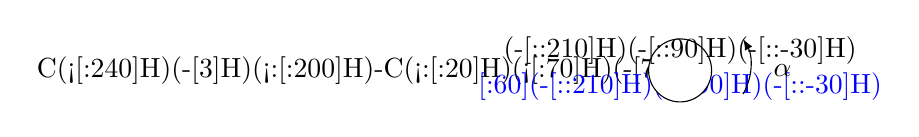
\begin{tikzpicture}[scale=1] 
        \node at(-4,0) {\chemfig{C(<[:240]H)(-[3]H)(<:[:200]H)-C(<:[:20]H)(<[:70]H)(-[7]H)} }; 
        \node [color=blue] at (0,-0.2) {\chemfig{[:60](-[::210]H)(-[::90]H)(-[::-30]H)}}; 
        \filldraw [fill=white](0,0) circle (0.4); 
        \node at (0,0.25) {\chemfig{(-[::210]H)(-[::90]H)(-[::-30]H)}}; 
        \draw [->,>=latex] (0.8,-0.3) arc (-30:30:0.7); 
        \node () at (1.3,0) {$\alpha$}; 
    \end{tikzpicture}
\end{minipage}%
%---------------------------------------------------------
\begin{minipage}[t]{0.45\linewidth}\centering
    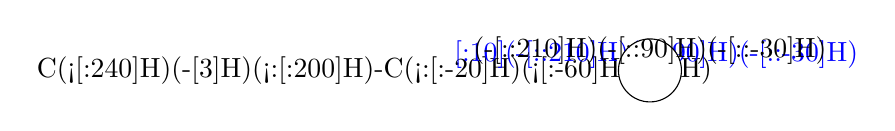
\begin{tikzpicture}[scale=1] 
        \node at(-3.5,0) {\chemfig{C(<[:240]H)(-[3]H)(<:[:200]H)-C(<:[:-20]H)(<[:-60]H)(-[1]H)} }; 
        \node [color=blue] at (0.08,0.2) {\chemfig{[:10](-[::210]H)(-[::90]H)(-[::-30]H)}}; 
        \filldraw [fill=white](0,0) circle (0.4); 
        \node at (0,0.25) {\chemfig{(-[::210]H)(-[::90]H)(-[::-30]H)}}; 
    \end{tikzpicture}   
\end{minipage}
\caption{Конформації молекули етану \ce{C2H6}}
\label{pic:Ethan_Conformation}
\end{figure}
%---------------------------------------------------------

Переріз ППЕ, який дає залежність енергії конформації від кута повороту $\alpha$ має вигляд, зображений на рис.~\ref{pic:Ethan_Conformation_E}.

%---------------------------------------------------------
\begin{figure}[h!]\centering
    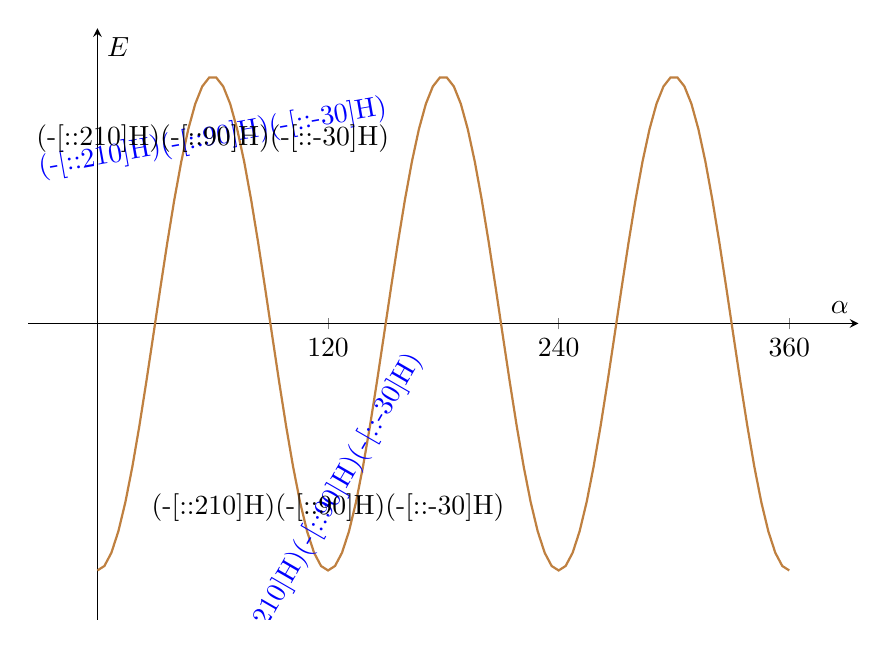
\begin{tikzpicture}
        \begin{axis}[
        axis lines = middle,
        xtick = {0, 2*pi/3,  4*pi/3 , 2*pi},
        xticklabels={0, $120$, $240$, $360$ },
        ytick = \empty,
        enlarge x limits=0.1,
        enlarge y limits=0.1,
        xlabel= {$\alpha$},
        ylabel= {$E$},
        width=\linewidth,
        height=0.7 5\linewidth,
        ]
            \addplot[domain=0:2*pi, samples=100, thick, brown]{-cos(3*deg(x))};
            \coordinate (max) at (axis cs:pi/3,0.75);
            \coordinate (min) at (axis cs:2*pi/3,-0.75);

                \node [color=blue, rotate=10] at (max) {\chemfig{(-[::210]H)(-[::90]H)(-[::-30]H)}}; 
                \node at (max) {\chemfig{(-[::210]H)(-[::90]H)(-[::-30]H)}}; 

                \node [color=blue, rotate around={60:(min)}, anchor = mid] at (min) {\chemfig{(-[::210]H)(-[::90]H)(-[::-30]H)}}; 
                \node [rotate around={0:(min)}, anchor = mid] at (min) {\chemfig{(-[::210]H)(-[::90]H)(-[::-30]H)}}; 
        \end{axis}
    \end{tikzpicture}
\caption{Залежність енергії конформації від кута повороту $\alpha$ в молекулі етану \ce{C2H6}}
\label{pic:Ethan_Conformation_E}
\end{figure}
%---------------------------------------------------------
З кривизною ППЕ пов'язані характер коливань ядер молекули і її жорсткість. Зокрема, другі похідні ППЕ поблизу мінімуму визначають частоти гармонічних коливань. Специфіка ППЕ для різних електронних станів молекули визначає і специфіку її спектральних характеристик.

Концепція ППЕ також відіграє важливу роль при розгляді механізмів і динаміки хімічних реакцій. Хімічна реакція на ППЕ зображується точкою, яка рухається по поверхні так, що при цьому зберігається повна енергія системи, а траєкторія переходу відповідає руху переходу від одного мінімуму, який відповідає реагентам до іншого мінімуму, що відповідає продуктам через сідлову точку. Сідлова точка при цьому відповідає перехідним станам. 

Важними характеристиками ППЕ як функції координати $E_\mathrm{el}(\vect{R}_1, \ldots, \vect{R}_K)$, є її векторний градієнт $\vect{g}$ і матриця Гессе $\mathbb{G}$ (гессіан). Градієнт повної енергії молекул (молекулярний градієнт) --- вектор виробничих функцій $E_\mathrm{el}(\vect{R}_1, \ldots, \vect{R}_K)$ за координатами, що визначається як

\begin{equation}\label{key}
    g_i = \frac{\partial E_\mathrm{el}(\vect{R}_1, \ldots, \vect{R}_K)}{\partial R_i}.
\end{equation}

Геометричний смисл молекулярного градієнта полягає в тому, що  показує виготовлення найшвидшого зростання ППЕ.

Матриця других похідних адіабатичного потенціалу за координатами (матриця Гесса або гессіан) $\mathbb{G}$ є:
\begin{equation}\label{key}
    G_{ij} = \frac{\partial^2 E_\mathrm{el}(\vect{R}_1, \ldots, \vect{R}_K)}{\partial R_i \partial R_j}.
\end{equation}

Гессіан у будь-якій точці конфігураційного простору визначає кривизну ППЕ. Гессіан є симетричною матрицею, оскільки $G_{ij} = G_{ji}$.

При лінійних перетвореннях системи координат гесіан може бути перетворений до діалогового виду: 
\[
    \mathbb{G} = \mathrm{diag}(G_{1}, G_{2}, \ldots, G_{K}).
\]

Діагональні елементи матриці, приведенної до діагональному виду, називаються власними значеннями цієї матриці. Важливою властивістю симетричної дійсної матриці є те, що її власні значення завжди є дійсними числами. У випадку несимметричних матриць, ця властивість не може виконуватися, навіть якщо все елементи вихідної матриці дійсні.

Координати конфігураційного простору, у яких матриця $\mathbb{G}$ має діагональний вигляд називаються власними векторами гессіана або нормальними координатами. Діагональні елементи гессіана, приведеного до діагонального вигляду називаються власними значеннями гессіана.

Важливою властивістю власних значень гессіана і нормальних координат є те, що вони визначають частоту і форму коливань молекули в даній точці ППЕ. Наприклад, якщо $\vect{R}_i$ --- декартові координати, то квадрат циклічної частоти коливання в даній точці ППЕ є: 
\[
    \omega^2_i = \frac{G_i}{m_A},
\]
де $m_A$~--- маса атома $A$.

З цієї точки зору багатоатомних молекул можна розглядати як набір незалежних гармонійних осциляторів, кожен їх яких має свою частоту коливання.

Обертання багатоатомної молекули можна представити як сукупність трьох незалежних ротаторів, кожен з яких має свою обертальну постійну, яка визначається геометрією молекули і має свою частоту коливання.

Для опису фізико-хімічних властивостей речовини на основі ППЕ, найбільш важливе значення мають її окремі точки, звані
стаціонарні точки ППЕ. Серед них найбільш важливі локальні мінімуми і сідлові точки (точки перехідних станів).

Локальні мінімуми ППЕ --- це точки, в яких виконується математичне умова мінімальності функції декількох змінних:
\begin{align}\label{}
    g_i(\vect{R}_1, \ldots, \vect{R}_K) &= 0, \\
    G_{i} (\vect{R}_1, \ldots, \vect{R}_K) &> 0.    
\end{align}

Друга умова означає, що всі власні значення матриці $\mathbb{G}$ (діагональні елементи матриці після приведення її до діагонального вигляду) є позитивними. У цьому випадку всі квадрати циклічних частот коливань молекули в точці локального мінімуму позитивні, а самі частоти --- дійсні позитивні числа.

Таким чином, знаходження локального мінімуму на ППЕ і розрахунок коливальних частот в цій точці дозволяє знайти всі термодинамічні функції речовини в стані ідеального газу. У разі хімічної реакції між цими речовинами, порівняння термодинамічних параметрів за законом Гесса дозволяє знайти термодинамічні параметри реакцій і константу рівноваги.

Сідлові точки ППЕ --- це точки, в яких одночасно виконуються три умови:

\begin{align}\label{}
    g_i(\vect{R}_1, \ldots, \vect{R}_K) &= 0, \\
    G_{1} (\vect{R}_1, \ldots, \vect{R}_K) &< 0.\\
    G_{i} (\vect{R}_1, \ldots, \vect{R}_K) &> 0.    
\end{align}

У цих точках вектор градієнта енергії дорівнює нулю, а кривизна позитивна в усіх напрямках, крім одного (і тільки одного), в якому вона негативна. Форма такої поверхні відповідає сідловині на перевалі між двома мінімумами, звідки і виникає її назву. Дуже часто сідлову точку називають точкою перехідного стану (ПС) хімічної реакції (або просто перехідним станом).

Важливо чітко уявляти, що ПС не є стійким станом молекули, в якому молекула існує якесь тривалий час. Характерний час, за який молекула «пролітає» цю точку дорівнює характерному часу міжатомних коливань, тобто $10^{-13}$~с. Тому існування молекули поблизу точки ПС не може бути зареєстровано звичайними експериментальними методами фізичної хімії, і тим більше ПС не може бути виділено у вільному стані. Один з експериментальних методів, який дозволяє реєструвати стану молекул зі швидкістю до $10^{-15}$~с --- це метод фемтосекундної спектроскопії, який дозволяє «зондувати» стани молекул в ході їх руху по ППЕ, в т.ч. і поблизу ПС. Однак цей метод має обмеження, що не дозволяють досліджувати довільні хімічні реакції, і в даний час подібні дослідження проведені тільки для невеликого числа фотохімічно-індукованих реакцій простих молекул в газовій фазі.

Важливість сідлових точок на ППЕ полягає в тому, що вони визначають вершину бар'єру між двома сусідніми локальними мінімумами. Завдяки цьому, через сідлову точку система може перейти з одного локального мінімуму в інший з найменшими витратами енергії (серед найближчих оточуючих точок), що означає протікання найбільш швидкої реакції перетворення однієї молекулярної структури в іншу. Таким чином, положення і енергія сідлової точки ППЕ визначає швидкість елементарного акту хімічної реакції. 

\emph{Пошук локальних мінімумів на ППЕ називається оптимізацією молекулярної геометрії. Він виконується шляхом багаторазового повторення квантовохімічного розрахунку енергії (і градієнта енергії) при варіації положень атомів.}

Початкова геометрія молекули вибирається на основі хімічних міркувань. Потім виконується Квантовохімічний розрахунок енергії і градієнта енергії, і спеціальний алгоритм визначає положення нової точки на ППЕ, енергія якої нижче. Якщо енергія даної точки або зміщення атомів дуже мала, пошук зупиняється. В іншому випадку робиться новий крок в напрямку зниження енергії.

Аналогічно виконується пошук перехідних станів. Однак в цьому випадку оптимізується не енергія, а сума квадратів градієнтів енергії, які в ПС повинні дорівнювати нулю. Крім того, в кінці оптимізації перевіряється, чи виконується умова ПС --- чи існує єдина уявна частота (єдине негативне значення гессіан).

%Цей образ відповідає фактично переходу від квантової до класичної картини.  

%Дійсно, точка, повна енергія $E$ якої фіксована, котиться по поверхні, що заповнює долини реагентів і продуктів. Її кінетична енергія уздовж так званого шляху реакції максимальна в порівнянні з іншими траєкторіями і вона швидко переходить з однієї долини в іншу. На цьому шляху зустрічається бар'єр, при русі через який  кулька сповільнюється, що відповідає наявності перехідного стану. Реальна картина класичного руху, а тим більше і квантового руху, без сумніву, суттєво складніша, проте при усередненні за всіма можливими траєкторіями, що буде відповідати безлічі окремих перетворень, картина виявляється близькою до вищевикладеної.


